\chapter{系统描述}

在本章中,我会详细描述系统中使用的概率图模型、随机游走算法以及2个方法的细节。
这2个方法是平行的,方法一是一个两阶段的方法,方法二是方法一的改版,其融合了方法一中的两步,这两个方法的输入和输出都是一样的。
输入都是 Web 表格和多知识库的实体数据,输出都是表格的实体链接结果,即表格中的字符串指称最终链接到的知识库中对应的参考实体。
换句话说,这2个方法中的任何一个都可以单独拿出来作为一个表格实体链接系统的核心算法。
我将这2个方法放在同一个系统中是为了可以更好地比较二者的效果差异。
在使用这个系统时,可以任意选择一个方法,然后得到已选择方法计算得到的实体链接结果。
目前实体链接的方法大体上可以分为3类:基于概率统计的方法,基于机器学习的方法和基于图模型的随机游走方法。
系统中的2个方法都是属于基于图模型的随机游走方法。
这类方法的思路与另外2类方法完全不同。
它主要利用字符串指称与实体之间、实体与实体之间的语义相关性来开展实体链接的工作。
它认为在位置上相邻的字符串指称往往具有语义相关性,比如表格中同行或者同列的指称描述的一般是同一个事物。
在我的方法中,会将字符串指称和知识库实体建模成一张概率图 (Probabilistic Graph Model),称之为实体消岐图 (Entity Disambiguation Graph),然后在这张图上运行随机游走 (Random Walk) 算法进行迭代消岐,直到图上实体节点的概率值收敛,最终得到链接结果。


\section{概率图模型}




\section{随机游走}




\section{方法一: 两步走}

方法一包含2个主要的步骤:首选使用各个单知识库进行实体链接,然后运行多知识库间的 ``sameAs'' 关系来优化单知识库的链接结果。

% Fig 3.1
\begin{figure}[htbp]
\centering
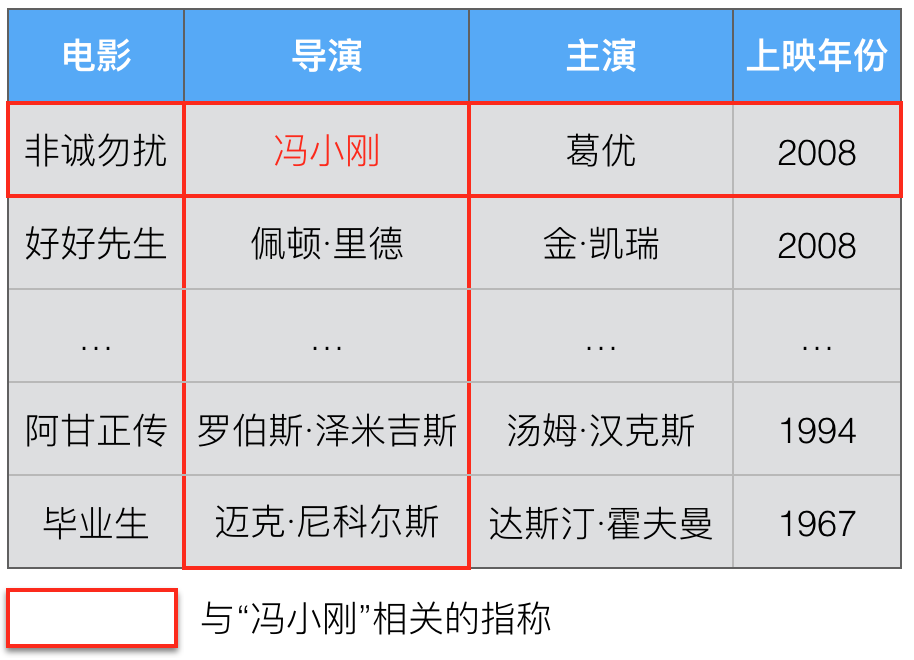
\includegraphics[width=0.6\textwidth]{img/relate}
\caption{一个表格同行同列中的指称具有语义相关性的例子}
\label{relate}
\end{figure}

\subsection{单知识库表格实体链接}

\noindent\textbf{指称识别}\newline
任何实体链接系统的第一步是识别出潜在的字符串指称,它们能够被链接到知识库中的参考实体。
给定来自输入的表格中每个单元格的文本内容,$t_q$,系统将 $t_q$ 中满足一定条件的最长的短语 $s$ 识别为潜在的指称。
这个条件就是对于某些实体 $e$,字符串 $s$ 能链接到该实体的概率 $P(e|s)$ 非零。
如果 $s$ 的长度小于 $t_q$ 的长度,系统会在 $s$ 之后发现长度最长的短语,并以此类推。
例如,对于一个单元格的文本 ``习近平 \& 彭丽媛'',系统会识别出到两个潜在的指称:一个是``习近平'',另一个是``彭丽媛''。\newline


\noindent\textbf{候选实体生成}\newline
对于表格单元格中的每个字符串指称,首先需要从给定的海量的知识库实体中找出一些可能成为该指称参考实体的实体,来缩小实体链接的范围。
这样的实体称为字符串指称的候选实体。这样的过程叫做生成候选实体。
在系统中,我讲每个指称分割到单词级别,所以每个指称能被表示为一个单词集合。
如果给定知识库中的一个实体 $e$ 或者 $s$ 在 BabelNet\cite{navigli2010babelnet} (一个全网域多语种同义词辞典) 中的一个同义词包含某个指称 $m$ 的分割单词集合中的至少一个单词,那么实体 $e$ 就被认为是指称 $m$ 的一个候选参考实体。
举个例子,字符串指称``苹果''有这样的一些候选实体:``苹果'',``苹果派'',``苹果 [水果]'',``苹果 [智能手机品牌]''。
候选实体生成的结果就是每个指称都可能指向一个候选实体集合。
在实际操作过程中,除了指称与实体的包含关系,我还考虑了二者之间的字符串相似度 (计算公式在后面会提到),设置了一个字符串相似度的阈值。
一般来说,与指称的字符串相似度很低的实体,很有可能表示的是跟指称完全不同的事物,即便它们有包含关系。
所以如果实体 $e$ 和指称 $m$ 的字符串相似度低于阈值,即使 $e$ 包含 $m$,也不将该实体 $e$ 添加进 $m$ 的候选实体集合。
比如,对于指称``苹果'',在知识库中有这样的一个实体``苹果红蜘蛛'',显然二者不可能相链接,虽然这个实体里包含了``苹果''二字,但是由于二者的字符串相似度太低,这样的实体就被剔除了。\newline

\noindent\textbf{实体消岐}\newline







\subsection{多知识库优化实体链接}

\begin{figure}[htbp]
\centering
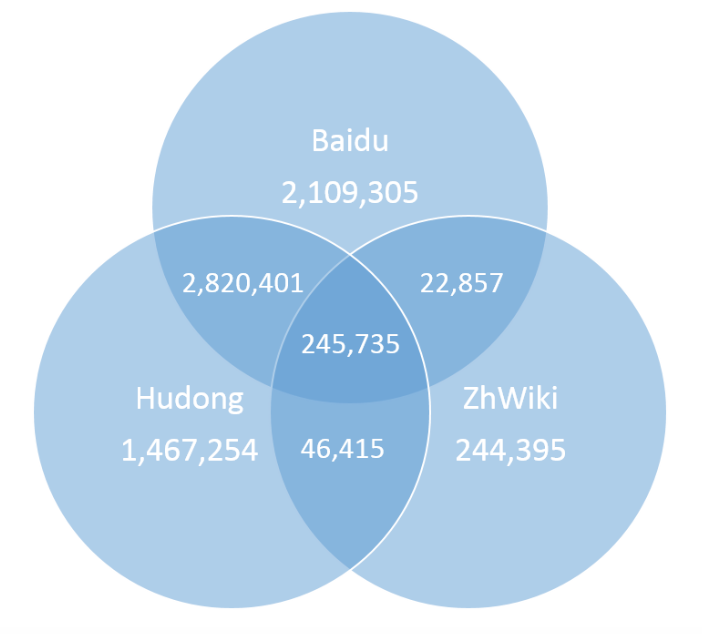
\includegraphics[width=0.4\textwidth]{img/zhishime_data}
\caption{Zhishi.me 数据统计}
\label{zhishime_data}
\end{figure}




\section{方法二: 融合}

\section{EL 与 sameAs 迭代学习}

\section{本章小结}
